\chapter{Theoretische Grundlagen}

\section{Aerodynamische Wirkweise des Rotors}
In der Welt der Windenergieerzeugung gibt es zwei grundlegende Bauformen von Windkraftanlagen: die Horizontalachsenwindkraftanlagen (HAWTs) und die Vertikalachsenwindkraftanlagen (VAWTs). Während Vertikalachsenanlagen bestimmte Vorteile in Bezug auf die Windrichtungsunabhängigkeit und die einfache Wartung aufweisen, haben sich Horizontalachsenwindkraftanlagen als die effizientere und weit verbreitete Option erwiesen. Diese Effizienz rührt von ihrer Fähigkeit her, höhere Energiemengen aus dem Wind zu extrahieren, insbesondere bei starken und konstanten Windverhältnissen, wie sie häufig in Offshore-Umgebungen vorkommen. Aufgrund dieser Überlegenheit in Bezug auf die Energieausbeute und die technologische Reife konzentriert sich diese Arbeit ausschließlich auf die Betrachtung und Analyse von Horizontalachsenwindkraftanlagen.

\begin{figure}[htbp] % Positionierungsoptionen: h=here, t=top, b=bottom, p=page of floats
    \centering % Zentriert das Bild
    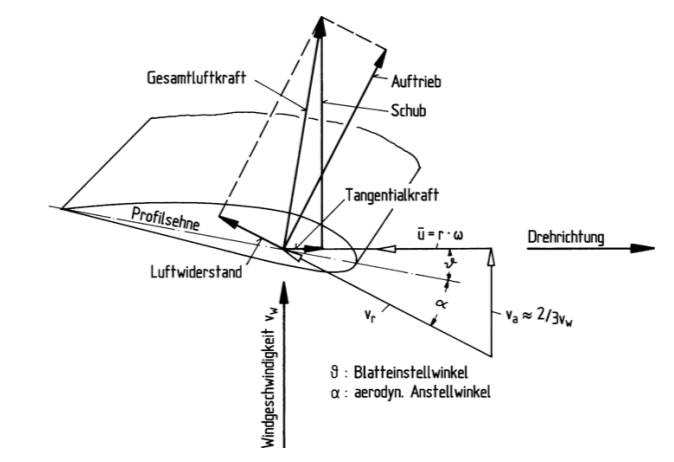
\includegraphics[width=0.8\textwidth]{figures/kraft_an_blatt.png} % Pfad zum Bild und Skalierung
    \caption{Kräfte am Rotorblatt resultieren in Drehmoment \cite{hau_physikalische_2016}} % Bildunterschrift
    \label{fig:kraft_an_blatt} % Label für Referenzen im Text
\end{figure}

Das zugrundeliegende physikalische Prinzip von HAWTs ist das gleiche wie bei Flugzeugflügeln: der Auftrieb.
Der Rotorblattquerschnitt ist so geformt, dass eine Differenz im Luftdruck zwischen der oberen und der unteren Seite des Rotorblattes entsteht, wenn Wind darüber strömt.
Die Unterseite des Rotorblattes erfährt einen höheren Druck als die Oberseite, was zu einer Auftriebskraft führt, die das Rotorblatt nach oben bzw. in Drehrichtung des Rotors zieht.
Dieser Auftrieb erzeugt um die Nabe des Rotors ein Drehmoment. Der Rotor dreht sich und treibt den Generator an.

\section{Kennzahlen}
Der Leistungsbeiwert \( C_P \) ist eine zentrale Kenngröße in der Aerodynamik von Horizontalachsenwindkraftanlagen (HAWAs) und quantifiziert das Verhältnis der nutzbaren mechanischen Leistung \( P \) einer Windturbine zur gesamten kinetischen Leistung des Windes \( P_{\text{wind}} \) im Rotorquerschnitt. Mathematisch ausgedrückt, ist \( C_P \) definiert als:

\begin{equation}
C_P = \frac{P}{\frac{1}{2} \rho A v^3}
\end{equation}

Hierbei repräsentiert \( \rho \) die Luftdichte, \( A \) die Querschnittsfläche des Rotors und \( v \) die Windgeschwindigkeit. Die Gleichung für \( P_{\text{wind}} \) reflektiert die Tatsache, dass die Leistung des Windes proportional zum Kubus der Windgeschwindigkeit ist.

Der Betzsche Grenzwert, eine theoretische Obergrenze für \( C_P \), wird durch die Betzsche Theorie festgelegt und ist auf maximal 59,3\% beschränkt. Dieser Wert, formal ausgedrückt als \( C_{P, \text{max}} = \frac{16}{27} \), basiert auf der Annahme, dass der Wind hinter der Turbine nicht vollständig zur Ruhe kommt, sondern noch eine Restgeschwindigkeit behält.
Diese Grenze repräsentiert das Maximum der Energieextraktion unter idealen, verlustfreien Bedingungen.

In der realen Anwendung sind Windturbinen verschiedenen Verlustquellen ausgesetzt. Zu diesen gehören Profilverluste, die durch Reibungswiderstand an den Rotorblättern entstehen, und induzierte Verluste, die durch die notwendige Änderung der Windrichtung hinter der Turbine verursacht werden. Diese Verluste sind besonders relevant für die Rotorblattgestaltung, da sie die aerodynamische Effizienz des Rotors direkt beeinflussen.

Fortschrittliche Windturbinendesigns streben danach, diese Verluste durch Optimierung der Rotorblattgeometrie und -ausrichtung zu minimieren. Dazu gehört die Feinabstimmung von Parametern wie Blattwinkel, Profiltiefe und -krümmung sowie die Berücksichtigung von Betriebsbedingungen wie Windgeschwindigkeit und -richtung. Die Anwendung von Computational Fluid Dynamics (CFD) und Blade Element Momentum (BEM)-Theorien spielt eine entscheidende Rolle bei der Entwicklung von Designs, die sich dem Betzschen Grenzwert annähern und gleichzeitig reale Betriebsbedingungen berücksichtigen.

\section{Aerodynamik eines Rotorblattes}
\subsection{Grundbegriffe}
\subsection{Kräfte und Kennzahlen}
\section{Methoden der Rotorblattauslegung}
\subsection{Auslegung nach Betz und Schmitz}
\subsection{Simulation mit Blatt-Element-Methode (BEM}
\section{Besonderheiten sehr kleiner Windkraftanlagen}